\documentclass{beamer}
\usepackage{graphicx}

\title[Crisis] % (optional, only for long titles)
{Computer Science 440 Project Presentation, Spring 2014}
\subtitle{Monday April 28th, 2014}
\author[Hawk Weisman, Dibyojyoti Mukherjee, Andreas Bach Landgrebe, Soukaina Hamimoune] % (optional, for multiple authors)
{Haw Weisman\inst{1} \and Dibyojyoti Mukherjee\inst{1}\\ \and Andreas Bach Landgrebe\inst{1} \and Soukaina Hamimoune\inst{2}}
\institute[Allegheny College, Department of Computer Science] % (optional)
{
  \inst{1}%
  Allgheny College\\
  Department of Computer Science
  \and
  \inst{2}%
  Al Akhawayn University\\
  Department of Computer Science
}
\date[April 28, 2014] % (optional)
{Team Remote}
\subject{Informatik}

\begin{document}
\frame{\titlepage}

\begin{frame}
\frametitle {\textbf{\textit Overview}}
\begin{itemize}
\item Remote Collab
\begin{itemize}
\item Online collaboration lets a group of people work together in real-time over the Internet
\item Allows the engaged collaborations to work together on a word processor documents or online presentations
\end{itemize}
\item SublimeText
\begin{itemize}
\item Cross-platform text and source code editor
\item Python-based plugin API
\item Extendable functionality with plugins
\item Cross platform (Windows, OS X, Linux)
\end{itemize}
\end{itemize}
\end{frame}

\begin{frame}
\frametitle {\textbf{\textit Architecture}}
\begin{itemize}
\item Client-Server Model
\begin{itemize}
\item Network architecture in which each computer or process on the network is either a client or a server.
\begin{itemize}
\item Client: Implemented as a plugin for SublimeText text editor
\item Server: Responsible for synchronization between clients
\end{itemize}
\item Both the Client and the Server will be released as a free open source software
\end{itemize}
\end{itemize}
\end{frame}

\begin{frame}
\frametitle {\textbf{\textit Architecture-Cont}}
	\begin{figure}
		\centering
		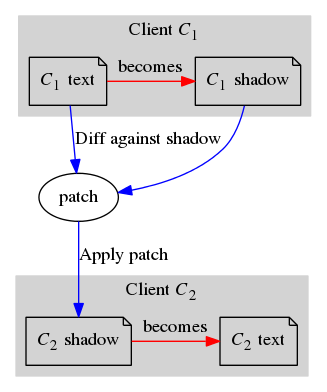
\includegraphics[width=0.5\linewidth]{diffsync.png}
		\caption{Dual-shadow differential synchronization}
		\label{fig:diffsync}
	\end{figure}
\end{frame}

\begin{frame}
\frametitle{\textbf{\textit Tools}}
\begin{itemize}
\item Python Socket Library
\begin{itemize}
\item[•]Remote communication between clients and the server
\end{itemize}
\item Sublime Text API
\begin{itemize}
\item Event driven functions used for system implementation. Functions called from the active buffer everytime the buffer is modified to perform a specific task.
\begin{itemize}
\item \textbf{\textit on\_modified(view)}
\item \textbf{\textit on\_modified\_async(view)}
\end{itemize}
\end{itemize}
\end{itemize}
\end{frame}

\begin{frame}
\frametitle {\textbf{\textit Implementation}}
\begin{itemize}
\item Python Programming Language
\item Git Hub
\item \url{http://teamremote.github.io/remote-sublime/}.
\item Andreas and Dibyo: networking
\item Sou and Hawk: Sublime Text Plug-in
\end{itemize}
\end{frame}



\begin{frame}
\begin{center}
\Huge Demonstration
\end{center}
\end{frame}



\end{document}


